\documentclass{article}
\usepackage[utf8]{inputenc}
\usepackage{pmboxdraw}
% Language setting
% Replace `english' with e.g. `spanish' to change the document language
\usepackage[english]{babel}

% Set page size and margins
% Replace `letterpaper' with`a4paper' for UK/EU standard size
\usepackage[letterpaper,top=2cm,bottom=2cm,left=3cm,right=3cm,marginparwidth=1.75cm]{geometry}

% Useful packages
\usepackage{amsmath}
\usepackage{graphicx}
\usepackage[colorlinks=true, allcolors=blue]{hyperref}
\usepackage{authblk}

\title{\textbf{LIDAR: Light Detection And Ranging}}
\author[1]{Dipayan Das}
\author[2]{Hardik Patil}
\author[3]{Srishti Keshari}
\affil[1]{Department of Metallurgical Engineering And Materials Science, IITB}
\affil[2]{Department of Metallurgical Engineering And Materials Science, IITB}
\affil[3]{Department of Chemistry, IITB}


\begin{document}
\maketitle


\section{Introduction}
As early as the invention of the laser in 1960, the development of a new kind of ranging system based on transmission and reception of light has been pursued, which included the adoption of already mature Radio Detection and Ranging (RADAR) principles. This new technique was then dubbed as LiDAR, that stands for Light Detection and Ranging. The main objective of both these techniques is to correctly detect and estimate the position of an object within a given scene, with swiftness and precision.

The original motivation for the development of LiDAR was the same as that of RADAR, military applications, mainly for target location, target recognition and weapon guidance purposes. From the 1960s onwards, several academic, industrial and military research efforts have been made by nations across all globe into this new laser ranging topic and with them, a great variety of useful applications were discovered.

\begin{figure}[h!]
\centering
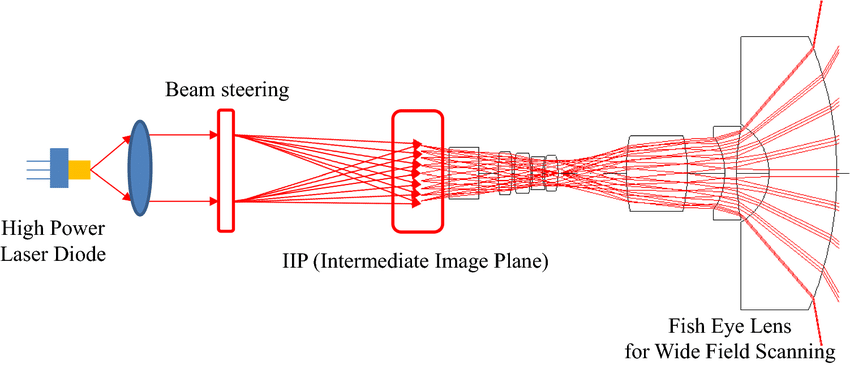
\includegraphics[width=1\textwidth]{Lidar Schematic.png}
\caption{\label{fig:xrd}Schematic diagram of a LIDAR sensing system\cite{lidarschematic}}
\end{figure}

Over the years, LiDAR has become more competitive compared to other sensing technologies, due to the continuous development of optical devices and its ability to achieve long-range and high spatial resolution, as optical wavelengths are capable of smaller diffraction angles for a given aperture size than microwave radar systems\cite{9435580}.

\section{LIDAR: Application}
LiDAR (Light Detection and Ranging) is a state of the art technology which measures the distance between objects and generates elaborate ancillary 3D visual maps of the relevant surrounding. It has a multitude of industrial applications. Some of the main categories of application of LiDAR are:
\begin{enumerate}
    \item Self-Driving Vehicles: LiDAR is one of the most important components for the functioning of self-driving vehicles because it enables them to constantly monitor the changing geographical landscape. Autonomous vehicles with LiDAR sensors can very accurately detect obstacles, road signs, lane markings, and even pedestrians making their navigation much safer. \cite{10192716}
\begin{figure}[h!]
\centering
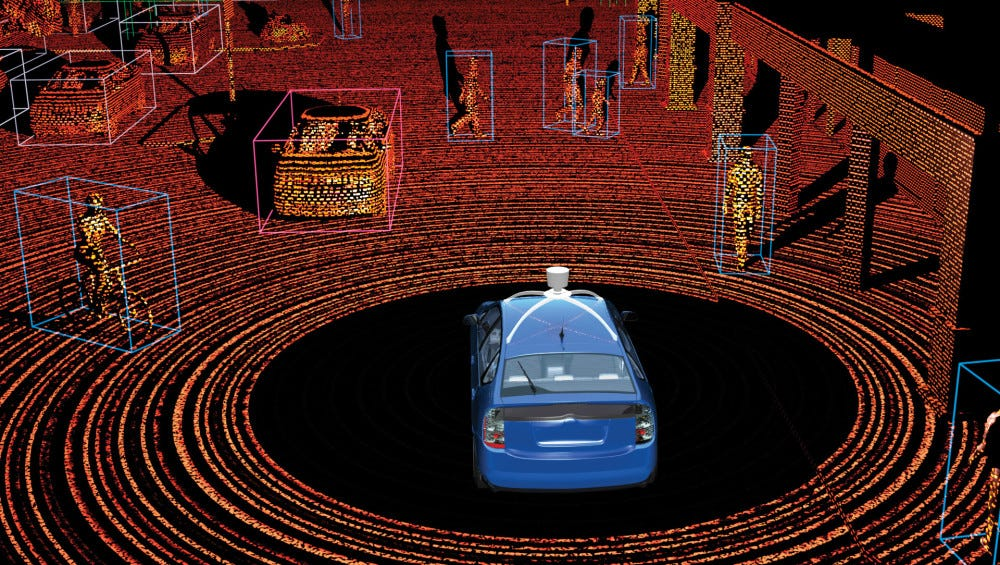
\includegraphics[width=1\textwidth]{selfdrive.jpg}
\caption{\label{fig:xrd}LiDAR in self-driving cars\cite{voyageIntroductionLIDAR}}
\end{figure}
    \item Geospatial Mapping and Surveying: LiDAR is comparatively more often applied in geospatial mapping and land surveying. It gives very precise vegetation, terrain and building topographic maps of extensive areas. Thus, it is needed for urban planning, flood modeling, and environmental assessment.\cite{7866543}
    \item Archaeology: LiDAR has transformed the field of archaeology especially in areas dominated by thick forests. It is capable of ‘seeing’ through trees and can be used to get detailed maps of ancient sites which were buried deep in vegetation. This helps in finding lost civilizations and regions with huge archaeological potential in remote areas.\cite{10167652}
    \item  Environmental Monitoring: LiDAR technology plays a vital role in the observation and management of natural resources. It is utilized to quantify deforestation, evaluate coastal erosion, monitor the growth of vegetation, and track wildlife habitats. Additionally, it is essential for disaster management, particularly in flood modeling and landslide prediction.
    \item Forestry: In the field of forestry, LiDAR is instrumental in measuring tree height, canopy density, and biomass, thereby providing comprehensive insights into forest composition and health. This technology supports forest management efforts, biodiversity conservation, and the assessment of carbon stocks.
    \item Mining: Within the mining sector, LiDAR is employed for topographic surveys, volume calculations, and safety inspections. It facilitates precise measurements of stockpiles and open-pit mining operations, while also aiding in the evaluation of site conditions.
    \item Construction \& Infrastructure: LiDAR is utilized in construction to develop accurate digital models of construction sites. It assists in monitoring project progress, identifying deviations from the original design, and ensuring proper alignment in infrastructure projects such as roads, bridges, and tunnels.
    \item Coastal \& Ocean Mapping: LiDAR is applied in bathymetric surveys to assess underwater topography. Coastal LiDAR is particularly beneficial for evaluating beach erosion, wave dynamics, and flood risks along coastal areas.
    \item Agriculture: In precision agriculture, LiDAR is used to generate three-dimensional models of farmland. This technology aids in crop monitoring, irrigation management, and the detection of changes in soil health or terrain, ultimately optimizing yields and minimizing resource consumption.
    
\end{enumerate}

\bibliographystyle{plain}
\bibliography{1,2,3,4,5,6,7,8,9}


\end{document}